\section{Entanglement in front of a thermal shield}\label{sec:5:thermal-entanglement}
The generation of entanglement between two particles depends heavily on variations in their initial placement, as seen in \cref{cha:entanglement-generation}.
Shield vibrations can effectively be understood to alter the separation and angle of the cat-state relative to shield, as depicted in \cref{fig:5:vibrating-translation-to-variations}.
\begin{figure}[!htbp]
  \centering
  \def\svgwidth{\textwidth}
  \input{./../figures/plate-vibration.pdf_tex}
  \caption{For a large ($r_s \gg R$) and locally linearizable shield, thermal vibrations with amplitude $z$ can be interpreted as a static shield where particle $A$ (shown in red) is positioned at $L+\Delta L$ with angle $\theta$ and particle $B$ at $L-\Delta L$ with angle $-\theta$. Both variations depend solely on the vibrational amplitude. At low vibrational frequencies ($1/\omega \approx t_\mathrm{max}$), the amplitude remains nearly static during an experimental run, with thermal fluctuations distributed around $\mean{\op{z}}=0$ and variance $\Delta \op{z}$ given by eq. \eqref{eq:5:amplitude-variance}. The particles are placed at a distance $r$ away from the shield's center. Especially the cases $r=0$ and $r\approx 0.527r_s$, where the gradient of the first mode $(1,0)$ is maximized, are considered.}
  \label{fig:5:vibrating-translation-to-variations}
\end{figure}
This approximation is only valid for shields significantly larger than the particle radius ($r_s \gg R$) and for low vibrational frequencies ($1/\omega \approx t_\mathrm{max}$), effectively capturing the impact of the first vibrational modes for small $l$ and $k$.
Especially the effect of the first mode $(1,0)$ can be put into the same framework from \cref{cha:entanglement-generation}. 
The interpretation is further supported by findings in \cref{sec:3:imperfect-plates}, showing that the Casimir interaction between a sphere and a tilted plane closely resembles that between a sphere and a flat plane.
Contrary to the problem considered in \cref{cha:entanglement-generation}, here only the thermal amplitude $z_{kl}$ is an independent random variable distributed around $\mean{z_{kl}}=0$ with a standard deviation $\Delta z_{kl}$ given by eq. \eqref{eq:5:amplitude-variance}. 
Variations in the particle-shield separation ($\Delta L$) and angle ($\theta$) are correlated to the vibration amplitude $z$.
For a large and linearizable shield, this can be understood as
\begin{equation}
  \theta = \arctan(z \abs{\nabla u}) \approx z \abs{\nabla u} \quad \text{and} \quad \Delta L = z \abs{u}
\end{equation}
where $\nabla u$ is the gradient of the vibrational mode's shape.
Performing similar calculations to those in \cref{cha:entanglement-generation}, the averaged density matrix $\mean{\rho}$, dependent on $\Delta z_{kl}$, can be derived (see \cref{apx:density-matrix-vibrating-plate}).
The resulting entanglement, quantified by logarithmic negativity as a function of temperature $T$ and particle-shield separation $L$, is given by eq. \eqref{eq:apx:en-thermal-shield} and shown in \cref{fig:5:entanglement-temperature}.
\begin{figure}[!htbp]
  \centering
  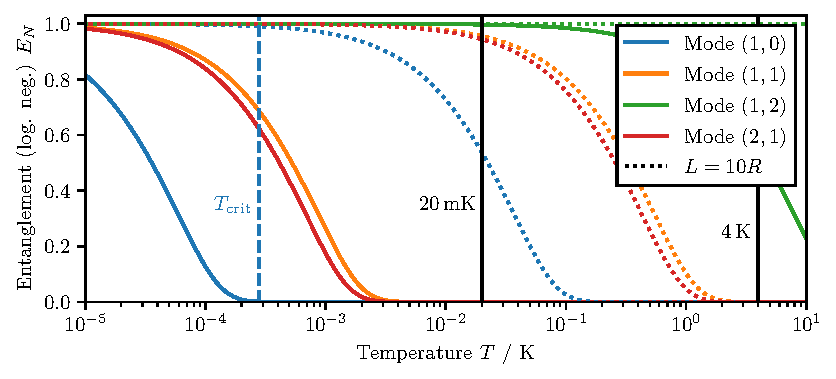
\includegraphics[width=\textwidth]{./../figures/vibrations/log-neg-shield-vibrations-T.pdf}
  \caption{Entanglement after a time $t_\mathrm{max}$ at different temperatures $T$. The particle (parameters given in \cref{tab:paramters}) is placed in front of a thermal shield, vibrating in selected modes $(k,l)$, at a position $r \approx 0.527 r_s$, where the effect of the first mode $(1,0)$ is maximized. The solid lines show the generated entanglement for $L=2R=20\si{\mu m}$ whereas the dashed lines show the entanglement for $L=10R$. At a critical temperature $T_\mathrm{crit} \propto L^4$, entanglement is lost.}
  \label{fig:5:entanglement-temperature}
\end{figure}
At typical experimental temperatures, entanglement in the presence of the mode $(1,0)$ is observable only at large particle-shield separations.
In fact, the critical temperature $T_\mathrm{crit}$ scales with the separation $L$ in the large-separation-limit (LSL) as (see \cref{eq:apx:decoherence-naive-vibration})
\begin{equation}
  T_\mathrm{crit} = \frac{\tilde{m} \omega^2_{kl}}{k_B}(\Delta z_\mathrm{crit})^2 \sim \left(\frac{L^5}{t_\mathrm{max}} \right)^2 \sim L^4 .
\end{equation}
The large separations required are consistent with previous findings in \cref{cha:entanglement-generation}, considering that the thermal amplitudes $\Delta z_{1,0} \approx 9 \times 10^{-11}\si{m}$ at $20\si{mK}$ are comparable with the critical values the variation in the shield-particle separation $\Delta L_\mathrm{crit}$.
Interestingly, these results are unaffected by the shield radius $r_s$, as long as $r_s \gg R$ and the vibrational mode can be locally linearized.
This invariance arises because the gradient $\abs{\nabla u} \sim 1/r_s$ and $\Delta z \propto r_s$ perfectly cancel, leaving $\theta$ independent of $r_s$. 
When the cat-state orientation is parallel to the shield, the system is very stable against variations in $\Delta L$, leaving the entanglement generation completely independent of $r_s$ in first order.

However, as seen in \cref{fig:5:entanglement-temperature}, the mode number $(k, l)$ significantly impacts entanglement generation.
Higher modes correspond to higher vibrational frequencies and smaller amplitudes $\Delta z$, with $T_\mathrm{crit}$ asymptotically scaling as $\mathcal{O}((k + l)^2)$. 
This behavior is presented in \cref{fig:5:T-crit-modes}.
\begin{figure}[!htbp]
  \centering
  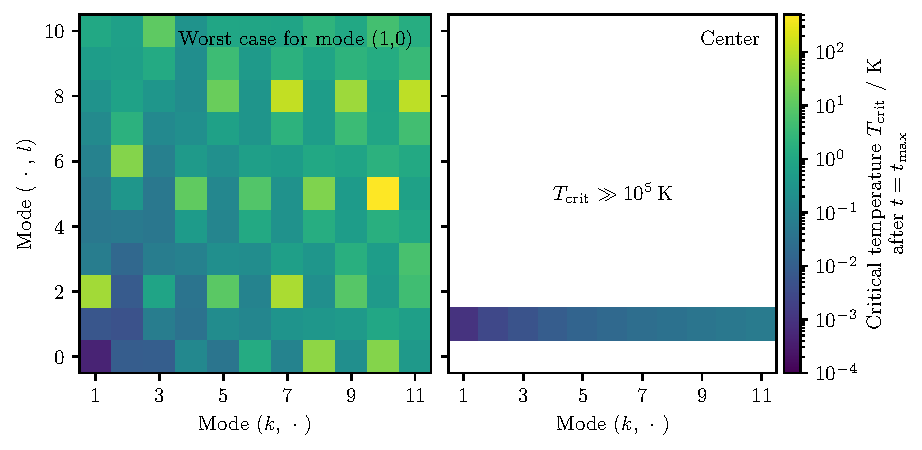
\includegraphics[width=\textwidth]{./../figures/vibrations/T-crit-modes.pdf}
  \caption{Critical temperature $T_\mathrm{crit}$, at which no entanglement is measurable anymore for different modes at a separation of $L = 2R = 2\si{\mu m}$. The shape of the vibrational modes is considered. The particle is either placed at the position of the highest gradient of mode $(1,0)$ (\textbf{left}) or in the center of the shield (\textbf{right}).}
  \label{fig:5:T-crit-modes}
\end{figure}
If the particle is positioned exactly at the center of the shield, only specific symmetric mode shapes with $l=2k+1,\ k\in\mathbb{N}_0$ can induce decoherence.
For $l > 1$, this decoherence effects become numerically indistinguishable from $0$.
If the particle is placed in the worst-case position for the first mode $(1,0)$, which corresponds to the point of maximum gradient $\abs{\nabla u}$ and thus the largest decoherence (approximately at $r \approx 0.527 r_s$), all modes are relevant.
It becomes evident, that only the first few vibrational modes significantly affect the entanglement generation.
The critical temperature for higher order modes increases and thus the generation of entanglement is not influenced by these vibrations even at reasonable high temperatures.

This naive method for calculating the decoherence induced due to the thermal shield is only accurate in the specific cases of a large and slow vibrating shield, as it requires the shield to be treaded as flat and tilted on the scale of the particle.
Furthermore, due to considering all modes separately, the combined effect is a huge overestimation, as each mode is treaded as maximally displaced simultaneously and no individual dynamics are accounted for.
In reality, the displacements of multiple simultaneously occurring modes can cancel each other partially out, reducing the overall decoherence.


\subsection{Analytic dynamics}\label{subsec:5:entanglement-analytical}
The effect of the thermal shield on entanglement generation between the two delocalized particles can be calculated analytically.
The Hamiltonian governing the interactions between the two particles with each other and with the thermal shield is given by
\begin{align}\label{eq:5:hamiltonian}
  \begin{split}
    \op{H} = &\sum_{\substack{m\in\{(k,l)\}\\ k \geq 1,\ l \geq 0}} \biggl\{ \hbar \omega_m \left(\op{a}^\dagger_m \op{a}_m + \frac{1}{2}\right) \\
    &+ g^{(1)}_\mathrm{A,m,Cas}(\op{a}_m + \op{a}^\dagger_m) \left( \ketbra{\psi^{(1)}_A} \otimes \identity \right)
     + g^{(2)}_\mathrm{A,m,Cas}(\op{a}_m + \op{a}^\dagger_m) \left( \ketbra{\psi^{(2)}_A} \otimes \identity \right) \\
    &+ g^{(1)}_\mathrm{B,m,Cas}(\op{a}_m + \op{a}^\dagger_m) \left( \identity \otimes \ketbra{\psi^{(1)}_B} \right)
     + g^{(2)}_\mathrm{B,m,Cas}(\op{a}_m + \op{a}^\dagger_m) \left( \identity \otimes \ketbra{\psi^{(2)}_B} \right)\biggr\} \\
    + g^{(1,1)}_\mathrm{Grav}&\ketbra{\psi^{(1)}_A \psi^{(1)}_B} + g^{(1,2)}_\mathrm{Grav}\ketbra{\psi^{(1)}_A \psi^{(2)}_B} \\
    + g^{(2,1)}_\mathrm{Grav}&\ketbra{\psi^{(2)}_A \psi^{(1)}_B} + g^{(2,2)}_\mathrm{Grav}\ketbra{\psi^{(2)}_A \psi^{(2)}_B}
  \end{split}
\end{align}
where the gravitational coupling
\begin{equation}
  g^{(ij)}_\mathrm{Grav} = \frac{G M^2}{L^{(ij)}}
\end{equation}
between the states $\ket{\psi^{(i)}_A}$ and $\ket{\psi^{(j)}_B}$ ($i,j = 1,2$) is determined by their separation $L^{(ij)}$ from eq. \eqref{eq:4:L-gravity}.
The shield's thermal vibrations have no influence on this coupling, hence the gravitational interaction is the same as already discussed in \cref{cha:entanglement-generation}.
Gravitational effects arising from the attraction due to the non-zero mass of the shield are omitted in these calculations because they are weaker by a factor of $10^7$ compared to the Casimir interactions, as calculated in \cref{subsec:5:shield-gravitation}.

The Casimir interaction strength $V^{(i)}_\mathrm{A(B),m,Cas}$ between the state $\ket{\psi^{(i)}_{A(B)}}$ and the shield is described by the term 
\begin{equation}
  V^{(i)}_\mathrm{A(B),m,Cas} = \frac{\hbar c \pi^3}{720}\left(\frac{\varepsilon_r - 1}{\varepsilon_r + 1}\right) \varphi(\varepsilon_r) \frac{R}{\left(\mathscr{L} + \op{z}_m u_m\left(r^{(i)}_{A(B)}\right)\right)^2}
\end{equation}
which is dependent on the mode $m$ and the mode displacement $\op{z}_m u_m$ at the position $r^{(i)}_{A(B)}$ of the cat-state, where $\op{z} = \sqrt{\hbar/2\tilde{m}\omega_m}(\op{a}_m + \op{a}^\dagger_m)$ is the amplitude of the vibration.
Expanding the term in first order in $\op{z}$ and ignoring the zeroth-order term, which is constant and thus equal to a global phase at the end of the calculations, the Casimir coupling in the Hamiltonian eq. \eqref{eq:5:hamiltonian} is given by
\begin{equation}
  g^{(i)}_\mathrm{A(B),m,Cas} = g_\mathrm{PFA} \frac{2 u_m(r^{(i)}_{A(B)})}{\mathscr{L}^3} \sqrt{\frac{\hbar}{2\tilde{m}\omega_m}}
  \quad \text{with} \quad 
  g_\mathrm{PFA} = \frac{\hbar c \pi^3 R}{720} \left(\frac{\varepsilon_r - 1}{\varepsilon_r + 1}\right) \varphi(\varepsilon_r) .
\end{equation} 
The combined system of the two particles $\rho_\mathrm{sys.} \in \mathcal{H}_\mathrm{sys.}$ and the thermal modes $\rho_\mathrm{th} = \bigotimes_m \rho_\mathrm{th, m} \in \mathcal{H}_\mathrm{th}$ evolves under the hamiltonian starting in the initial state $\rho_0 = \rho_\mathrm{th} \otimes \rho_\mathrm{sys.}$. 
The initial state of the two particles $\rho_\mathrm{sys.}$ is given by eq. \eqref{eq:2:initial-state} and $\rho_\mathrm{th,m}$ is the thermal state of vibrational mode $m$, which can be represented either in the number basis $\{\ket{n}\}$ or in the coherent state basis $\{\ket{\alpha}\}$ as \cite{Steiner_2024}
\begin{equation}
  \rho_\mathrm{th,m} = \frac{1}{Z} \sum_{n=1}^\infty e^{-\beta \hbar \omega_m (n + 1/2)} \ketbra{n} = \int \dd \alpha^2 \frac{1}{\pi \bar{n}} e^{-\frac{\abs{\alpha}^2}{\bar{n}}} \ketbra{\alpha} .
\end{equation} 
Here, $Z = \tr e^{-\beta \hbar \omega_m (\op{n}+1/2)} = e^{-\beta \hbar \omega_m/2}/(1-e^{-\beta \hbar \omega_m})$ is the partition function and $\bar{n} = 1/(e^{\beta \hbar \omega_m} - 1)$ is the average thermal occupation number of mode $m$ at temperature $T$. 

After time $t$, tracing out the thermal shield yields the evolved two-particle system
\begin{equation}
  \rho_\mathrm{sys.}(t) = \tr_\mathrm{th}\left(\op{U}(t) \, \rho_0 \, \op{U}^\dagger(t)\right) .
\end{equation}
The time evolution is computed in \cref{apx:thermal-shield-time-evolution} and is given by
% \begin{equation}
%   \rho_\mathrm{system}(t) = \frac{1}{4} \begin{pmatrix}
%     1 & e^{i\phi_{11,12}} e^{-\gamma_{11,12}} & e^{i\phi_{11,21}} e^{-\gamma_{11,21}} & e^{i\phi_{11,22}} e^{-\gamma_{11,22}} \\
%     & 1 & e^{i\phi_{12,21}} e^{-\gamma_{12,21}} & e^{i\phi_{12,22}} e^{-\gamma_{12,22}} \\
%     \multicolumn{2}{c}{\multirow{2}{*}{c.c}} & 1 & e^{i\phi_{21,22}} e^{-\gamma_{21,22}} \\
%     & & & 1 \\
%   \end{pmatrix}
% \end{equation}
\begin{equation}
  \rho_\mathrm{system}(t) = \frac{1}{4} \begin{pmatrix}
    1 & e^{i\phi_{11,12}} e^{-\gamma_{11,12}} & e^{i\phi_{11,21}} e^{-\gamma_{11,21}} & e^{i\phi_{11,22}} e^{-\gamma_{11,22}} \\
    e^{i\phi_{12,11}} e^{-\gamma_{12,11}} & 1 & e^{i\phi_{12,21}} e^{-\gamma_{12,21}} & e^{i\phi_{12,22}} e^{-\gamma_{12,22}} \\
    e^{i\phi_{21,11}} e^{-\gamma_{21,11}} & e^{i\phi_{21,12}} e^{-\gamma_{21,12}} & 1 & e^{i\phi_{21,22}} e^{-\gamma_{21,22}} \\
    e^{i\phi_{22,11}} e^{-\gamma_{22,11}} & e^{i\phi_{22,12}} e^{-\gamma_{22,12}} & e^{i\phi_{22,21}} e^{-\gamma_{22,21}} & 1 \\
  \end{pmatrix}
\end{equation}
with the decoherence terms
\begin{equation}\label{eq:5:analytical-decoherence}
  \gamma_{ii',jj'} = \sum_m \frac{4}{\hbar^2\omega_m^2} \abs{(g^{(i)}_\mathrm{A,m,Cas} + g^{(i')}_\mathrm{B,m,Cas}) - (g^{(j)}_\mathrm{A,m,Cas} + g^{(j')}_\mathrm{B,m,Cas})}^2 \sin^2\left(\frac{\omega_m t}{2}\right) \left[\bar{n} + \frac{1}{2}\right]
\end{equation}
and the phases
\begin{multline}\label{eq:5:analytical-phases}
  \phi_{ii',jj'} = \sum_m \frac{1}{\hbar} \left( g^{(ii')}_\mathrm{Grav} - g^{(jj')}_\mathrm{Grav} \right) t \\
  + \frac{\sin(\omega_m t)+\omega_m t}{\hbar^2\omega_m^2}\left[(g^{(i)}_\mathrm{A,m,Cas} + g^{(i')}_\mathrm{B,m,Cas})^2 - (g^{(j)}_\mathrm{A,m,Cas} + g^{(j')}_\mathrm{B,m,Cas})^2\right] .
\end{multline}
At $T=0$, decoherence terms persist, but their effect is only significant for strong Casimir interactions (e.g., small separations $L\approx R$).
The decoherence scales as $\gamma \propto \omega_m^{-4}$ from which the asymptotic dependence on the modes $\mathcal{O}((k+l)^{-8})$ directly follows.
It is therefore possible to estimate the combined effect of the first $N$ modes as
\begin{equation}\label{eq:5:effect-of-a-mode}
  \sim \frac{1}{\zeta(8)} \sum_{n=1}^{N} \frac{1}{n^8}
\end{equation}
where $\zeta$ is the Riemann zeta function. The sum eq. \eqref{eq:5:effect-of-a-mode} converges very fast to $1$, even for small $N$.
At specific times $t=2\pi k/\omega_m, \ k\in\mathbb{N}$, the decoherence from mode $m$ vanishes, leading to entanglement values close to the ideal case, aligning with the findings in Ref. \cite{Pedernales_2022}.
This periodic behavior is confirmed in \cref{fig:5:entanglement-time-single-mode}, showing a measurable amount of entanglement only close to these specific times.
\begin{figure}[!htbp]
  \centering
  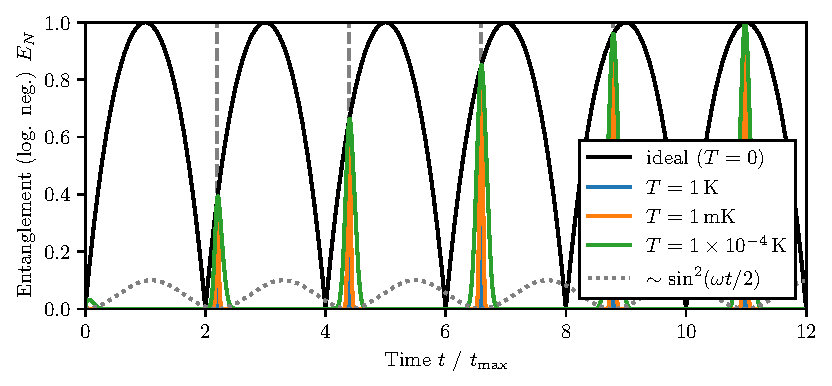
\includegraphics[width=\textwidth]{./../figures/vibrations/entanglement-hamiltonian.pdf}
  \caption{Entanglement dynamics in front of a thermal shield in mode $(1,0)$ at different temperatures. Only at specific times $2\pi k / \omega_{1,0} \approx k\times 576\si{ms},\ k\in\mathbb{N}$, entanglement is observable. This aligns with the findings in Ref. \cite{Pedernales_2022}. The particle and shield parameters are taken from \cref{tab:paramters}.}
  \label{fig:5:entanglement-time-single-mode}
\end{figure}
The full width at half maximum (FWHM) of these observed peaks is approximated by
\begin{equation}
  \mathrm{FWHM} \approx \frac{4}{\omega}\sqrt{\frac{\log 2}{\gamma}} \propto \frac{1}{\sqrt{\bar{n}}} \sim \sqrt{\omega/T},
\end{equation}
getting smaller at higher temperatures.

The resulting decoherence of multiple modes is given by the sum of all individual modes, where the contributed effect decays rapidly with the mode number, as seen in eq. \eqref{eq:5:effect-of-a-mode}.
Entanglement as seen without the shield is never reachable due to the quasi-periodicity of the system. The frequency ratios $\omega_i/\omega_j \notin \mathbb{Q}$ for $i\neq j$ \footnote{While not rigorously proven, this conclusion is supported by the transcendental nature of the zeros of the Bessel functions \cite{Lorch_1995}.} prevent exact repetition of the resulting sinusoidal summation.
The entanglement dynamics of the first 50 vibrational modes combined are shown in \cref{fig:5:entanglement-multiple-modes} .
\begin{figure}[!htbp]
  \centering
  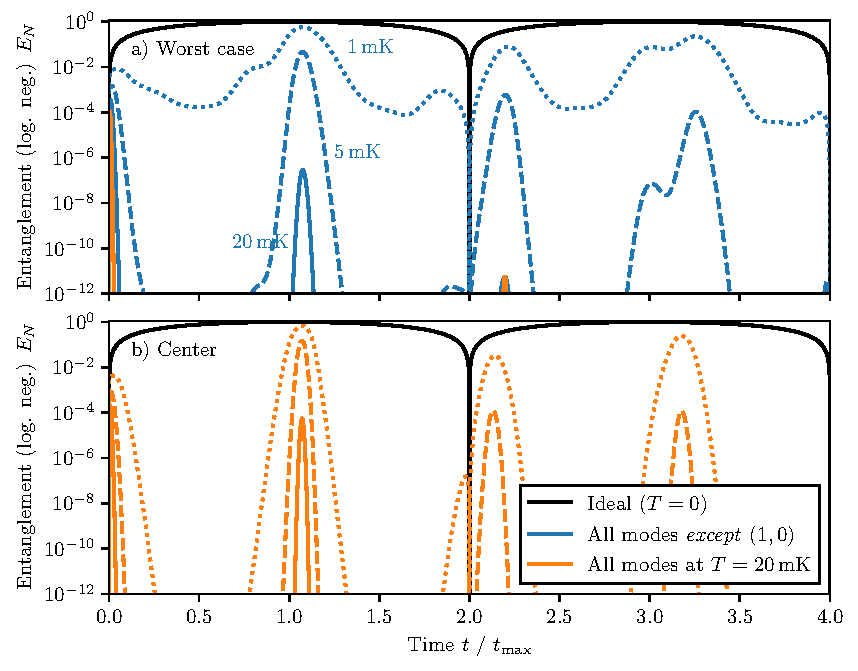
\includegraphics[width=\textwidth]{./../figures/vibrations/entanglement-dynamics-all-modes.pdf}
  \caption{Entanglement dynamics in front of a thermal shield. \textbf{Orange}: The first 50 modes have been used in the numeric calculation. The effect of all remaining modes is around $1.7 \times 10^{-11}\,\%$. \textbf{Blue}: Results excluding the $(1,0)$ mode at varying temperatures ranging from $1\si{mK}$ up to $20\si{mK}$. In part \textbf{a)} the particles are placed in the worst-case position of the shield where the effect of the mode $(1,0)$ is maximized. In \textbf{b)} the particles are placed in front of the center of the shield. The parameters used are taken from \cref{tab:paramters}.}
  \label{fig:5:entanglement-multiple-modes}
\end{figure}
This figure highlights the dominant contribution of the first mode $(1,0)$, with realistically measurable entanglement primarily occurring at $t = 2 \pi/\omega_{1,0}$.
Even for temperatures as low as $20\si{mK}$, entanglement remains minimal due to large decoherence.
Increasing the particle-shield separation reduces Casimir coupling $g_\mathrm{Cas} \propto \mathscr{L}^{-3}$ and hence reducing the decoherence while simultaneously slowing gravitational entanglement generation down ($t_\mathrm{max} \propto L^3$).
The combined effect is therefore qualitatively given by $\gamma \propto g_\mathrm{Cas}^2 \sin^2(t) \propto L^{-6} \sin^2(L^3) \xrightarrow{L \gg R} 0$, suggesting that no decoherence is present at large separations.
The dependence of entanglement on the particle-shield separation at two specific points in time is shown in \cref{fig:5:entanglement-thermal-shield-L}.
\begin{figure}[!htbp]
  \centering
  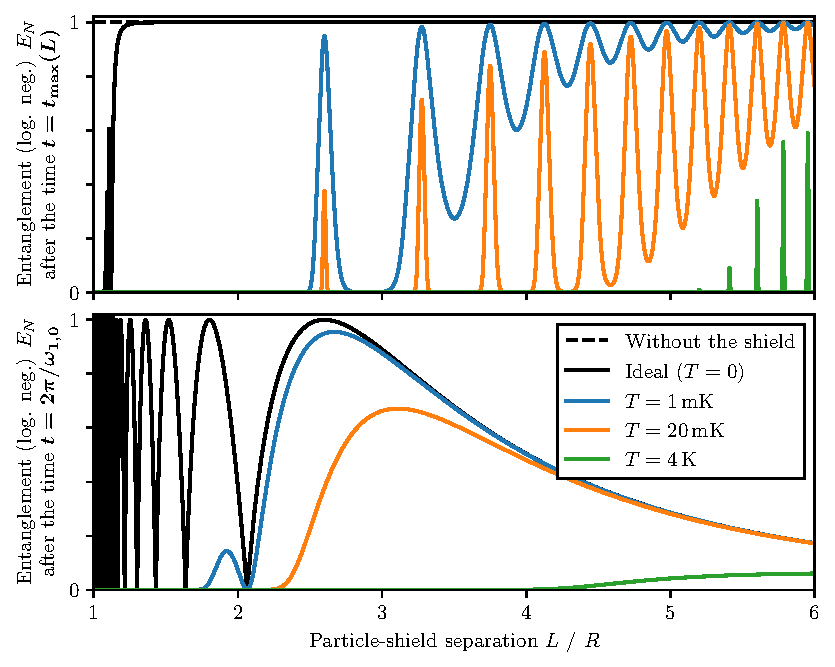
\includegraphics[width=\textwidth]{./../figures/vibrations/all-modes-entanglement-L.pdf}
  \caption{Entanglement generation for different particle-shield separations $L > R$ and different temperatures at times $t_\mathrm{max}(L)$ (eq. \eqref{eq:4:t-max}) (\textbf{top}) and $t = 2\pi/\omega_{1,0}\approx 576\si{ms}$ (\textbf{bottom}). Calculations use parameters from \cref{tab:paramters} and the particles are placed in the worts-case position in front of the shield, where the effect of the mode $(1,0)$ is maximized.}
  \label{fig:5:entanglement-thermal-shield-L}
\end{figure}

By measuring after a time $t_\mathrm{max}(L)$ (with $t_\mathrm{max}(20\si{\mu m}) \approx 258\si{ms}$), in the ideal scenario without the shield, a maximally entangled state with $E_N = 1$ is observed.
Although $2\pi/\omega_{1,0}$ is constant in time, $t_\mathrm{max}$ increases with $L$, creating specific separations (e.g. for $L\approx 2.6R$) where the two times align, enhancing observability.
For even larger $L$, decoherence effects eq. \eqref{eq:5:analytical-decoherence} diminish, making entanglement measurable even at higher temperatures.

By measuring at the time $2\pi/\omega_{1,0} \approx 576\si{ms}$ where the decoherence of the first mode almost vanishes, entanglement can be observed by increasing the particle-shield separation.
However, measuring at a constant time independent of $L$ limits the maximum of possibly reachable entanglement as the gravitational entanglement rate slows down and increasing $t_\mathrm{max}$.

The radius of the shield also has a large impact on entanglement generation. Smaller shields with larger mode frequencies result in a decreased and faster oscillating decoherence $\gamma \propto \sin^2(\omega) 1/\omega_m^2$.
The time between the points, where the decoherence effect of the first mode almost vanishes (i.e. every $\Delta t = 2\pi/\omega_{1,0} \propto r_s^2$), decreases for smaller shields and thus making entanglement measurable more frequently at almost any point in time.
Numeric calculations show, that even for shields as large as $r_s = 5\si{mm}$, entanglement of around $E_N \lesssim 1$ can be measured at $T = 20\si{mK}$ even at close separations (see \cref{fig:apx:entanglement-thermal-shield-rs-5mm} and \cref{fig:apx:entanglement-thermal-shield-rs}).

\subsubsection*{Indirect entanglement through the shield}

Examining the phases $\phi_{ii',jj'}$ in eq. \eqref{eq:5:analytical-phases} reveals that, similar to the gravitational force, the Casimir interaction between the particle and the shield can induce entanglement between the particles. This occurs as both particles couple to the shield via Casimir interactions, enabling indirect interaction between them.
However, the resulting amount of entanglement is very small, as evident from the dependence on $1/\hbar^2$ in eq. \eqref{eq:5:analytical-phases}.
While negligible at larger separations, Casimir-induced indirect entanglement could become significant at very small distances where the Casimir forces are much stronger than the gravitational interaction. 
This is particularly relevant if the entanglement generated via Casimir interactions approaches that due to gravity. 
The relative strength can be estimated by comparing the term corresponding to the gravitational interaction with the Casimir terms in eq. \eqref{eq:5:analytical-phases}:
\begin{align}
  g_\mathrm{Grav} t &\gtrsim \frac{\sin(\omega_m t) + \omega_m t}{\hbar \omega_m^2} g_\mathrm{Cas}^2 \\
  \Longrightarrow \quad 
  \frac{G M^2}{2L} &\gtrsim g_\mathrm{PFA} \frac{1}{\mathscr{L}^3} \sqrt{\frac{\hbar}{2\tilde{m}\omega_m}}
\end{align}
where $\mean{\sin(\omega t)} = 0$ was averaged.
Using the parameters for the particles and the shield from \cref{tab:paramters}, the lower bound for the separation is given by $L > 1.29\times 10^{-5}\si{m}\approx 1.3 R$. For separations $L \gtrsim 2.7R$, gravitational entanglement becomes $100$ times stronger than entanglement due to Casimir interactions.
These separation limits are most likely fulfilled either way considering the results from the previous chapters, thus indirect entanglement can be neglected in all practical circumstances.



\subsection{Small shields}
A small shield can only block the direct Casimir interactions between the particles $A$ and $B$, hence it can only be used if no other forms of electromagnetic interactions between the particles such as Coulomb coupling are present.
For very small shields in the size of the particles $r_s \sim R + \Delta x / 2$, the above considerations are not fully applicable, as they assume the linearization of the vibrational mode at the particle's scale.
The vibrations of the shield and the resulting vibrational modes substantially alter the Casimir potential, which is no longer determined solely by the interaction between a perfectly flat shield and a spherical particle. 
Deformations can no longer be approximated locally as a flat, tilted plate; instead, the shape of the vibrational mode must be accounted for. 
As discussed in \cref{sec:3:imperfect-plates}, deformations, such as those resembling the first vibrational mode, significantly impact the resulting Casimir potential which is, in the proximity-force approximation, bounded by an interaction equivalent to that between a sphere and a plate with separation $\mathscr{L} \pm \Delta z$.

In the temporal domain, vibrational frequencies scale quadratically with the shield size, $\omega \propto 1/r_s^2$, which results in the measuring process being multiple times longer than a single vibrational period. 
Consequently, Casimir interactions are averaged over time, leading to an effectively planar and flat shield.
This agrees with the findings in the previous section and the results shown in \cref{fig:apx:entanglement-thermal-shield-rs-5mm}, where smaller shields exhibit drastically reduced decoherence effects.

Similar reasoning applies to higher vibrational modes in arbitrarily large shields. 
These modes, characterized by high frequencies and a roughly uniform  distribution of deformations, effectively average out the Casimir interactions in the temporal domain as well as because of the findings in \cref{sec:3:imperfect-plates}, preserving entanglement.
